\documentclass{article}

\usepackage[margin=1in]{geometry}
\usepackage{setspace}
\usepackage{graphicx}
\usepackage{amsmath}

\begin{document}
\onehalfspacing
\begin{titlepage}
	\clearpage\thispagestyle{empty}
	\centering
	\vspace{1cm}
		
	\rule{\linewidth}{1mm} \\[0.5cm]
	{ \Large \bfseries ISyE 6740 - Summer 2022\\[0.2cm]
		Final Report}\\[0.5cm]
	\rule{\linewidth}{1mm} \\[1cm]
	
		\begin{tabular}{l p{5cm}}
		\textbf{Team Member Names:} Matthew Rand, Changhong Guan &   \\[10pt]
		\textbf{Project Title:} Optimizing Initial Launch of eVTOL Operations &  \\[10pt]
		\end{tabular} 
	
	\tableofcontents
	
\end{titlepage}

\section{Problem Statement}
		
Urban air mobility is a fast-emerging field that is poised to revolutionize the transportation industry. Multiple companies across the world contend to bring access to a network of eVTOL aircraft that will allow for intra-city travel for the price of an Uber. While the initial economics limit the market and feasibility of the product, as the industry grows, the price point will continue to drop and expand access to broader markets across the country and across the globe.

When considering the phased growth of an industry, it becomes necessary to determine the right market dynamics to target for initial operations that properly balances growth potential with a high probability of user adoption. The United States is the perfect incubator for such an industry, with the largest cities in America experiencing high-growth in geographically constrained regions. However, not all cities developed equally. Not only do population densities vary city to city, but access to public transportation, traffic congestion, and wealth disparities change market dynamics.

A nascent industry must pick and choose its launch markets very carefully. As such, this problem is well-suited for an optimization algorithm that can determine the ideal set of launch parameters and determine which locations boast the best opportunity for success.

\section{Data Source}

\subsection{US Commute Flow Data}
This data set is provided by the United States Census Bureau. The data is relevant as of 2015. This data set is used to find which major metropolitan cities has the most and possibly the worst commute situation, that makes it ideal candidate for exploring eVTOL aircraft network implementation to alleviate commute nightmare. After descending sort on commute count, Los Angeles County (Los Angeles), Cook county (Chicago) and Harris County (Houston), rank top 3 the most commute counties. And we picked Los Angeles County or greater Los Angeles area for further exploration.

\subsection{Locations of Available US Heliports and Airports}
This dataset is provided by the Federal Aviation Administration and includes the latitude and longitude of all airports and heliports in the United States. Here we define vertiports as heliports and airports combined. We are assuming that to save on capital expenditure, initial operations will focus on retrofitting current aviation locals in lieu of developing brand new ones.

\subsection{Neighborhood Geospatial Data of Greater Los Angeles}
By using geopandas, geospatial data allows us to accurately map the Greater Los Angeles region and represent the physical location of different neighborhood centers given their boundary, centroids and area. It also provides population density for each neighborhood, from which we extrapolated potential commute need for each neighborhood as well.

\subsection{Average Commute duration by time of data for Greater Los Angeles}
To approximate the average commute by potential customers, we utilized the U.S. Census Bureau's 2019 American Communities Survey 1-year Public Use Microdata Area (PUMA) sample. This sample was collected from over 800 respondents in 69 regions corresponding to 160 neighborhoods in the Greater Los Angeles Metro region and collected demographic information, as well as information on transportation and commuting. We believed that 2019 would be the most accurate sampling to current conditions given it was the last pre-pandemic survey conducted. 

\section{Methodology}
Our ultimate goal is to evaluate the economic viability of launching urban air mobility operations as an alternative to current ride-hailing solutions, or even personal vehicle usage. To do so, we must establish a market need by identifying the cost of travel for individuals in different geographic locations, create a comparative model for idealized urban air mobility operations, and determine the difference in cost that could be captured by the urban air mobility industry.

We will focus on determining the maximum daily profitability of a hypothetical eVTOL company in the Greater Los Angeles Metro area,  a region well-publicized in the industry as a target for initial operations due to the density and wealth of the population. Los Angeles is also well-known for having terrible traffic conditions, so an airborne alternative to typical transportation modes is a desirable solution seeing as current terrestrial solutions have been ineffective at reducing traffic in the region. We corroborated this sentiment using US total commute data, where we sorted by the number of commuters for each county, to find greater LA area is the heaviest in commute traffic, and thus worth exploring.

While important to select initial markets based on both population and wealth, its also important to note that it can be expensive to build the infrastructure required to launch operations. Therefore, we will utilize the FAA's database of existing airports and heliports to initialize cluster centers, since utilizing existing infrastructure dramatically reduces launch costs.

\subsection{Clustering}

We can begin by running a cluster analysis on Geo-spatial data of over 200 communities and neighborboods from the LA area to determine how many serviceable communities there are, how large those communities are, and map those regions against the FAA airport/heliport database to determine just how many existing locations may be able to service a cluster. We initialize cluster centers on different combinations of vertiport locations to pre-condition the results so that clusters are located nearby to existing infrastructure. 

This may lead to a sub-optimal result when considering the clustering analysis in isolation, however, business needs necessitate cost-reduction for capital expenditures to lower the barrier to entry and to beginning revenue-generating operations. However, since clustering is an unsupervised algorithm and given that there many permutations of potential clusters, this technique ensures that any particular cluster center becomes a viable option rather than a theoretical best-case scenario.

Given the clusters determined by the algorithm, we will import the commute data, match clusters with their commute data, and generate two data sets.

\subsubsection{Preprocessing: Geopandas}
Geopandas library is used to work with Geo-spatial data, in our case, in geojson format. After calculating the centroid of each neighborhood, we plot the Los Angeles area we are interested in, in Figure \ref{fig:proj01}, with red dots representing neighborhood centers and dark yellow dots representing currently available vertiports.

\begin{figure}[ht]
\centering
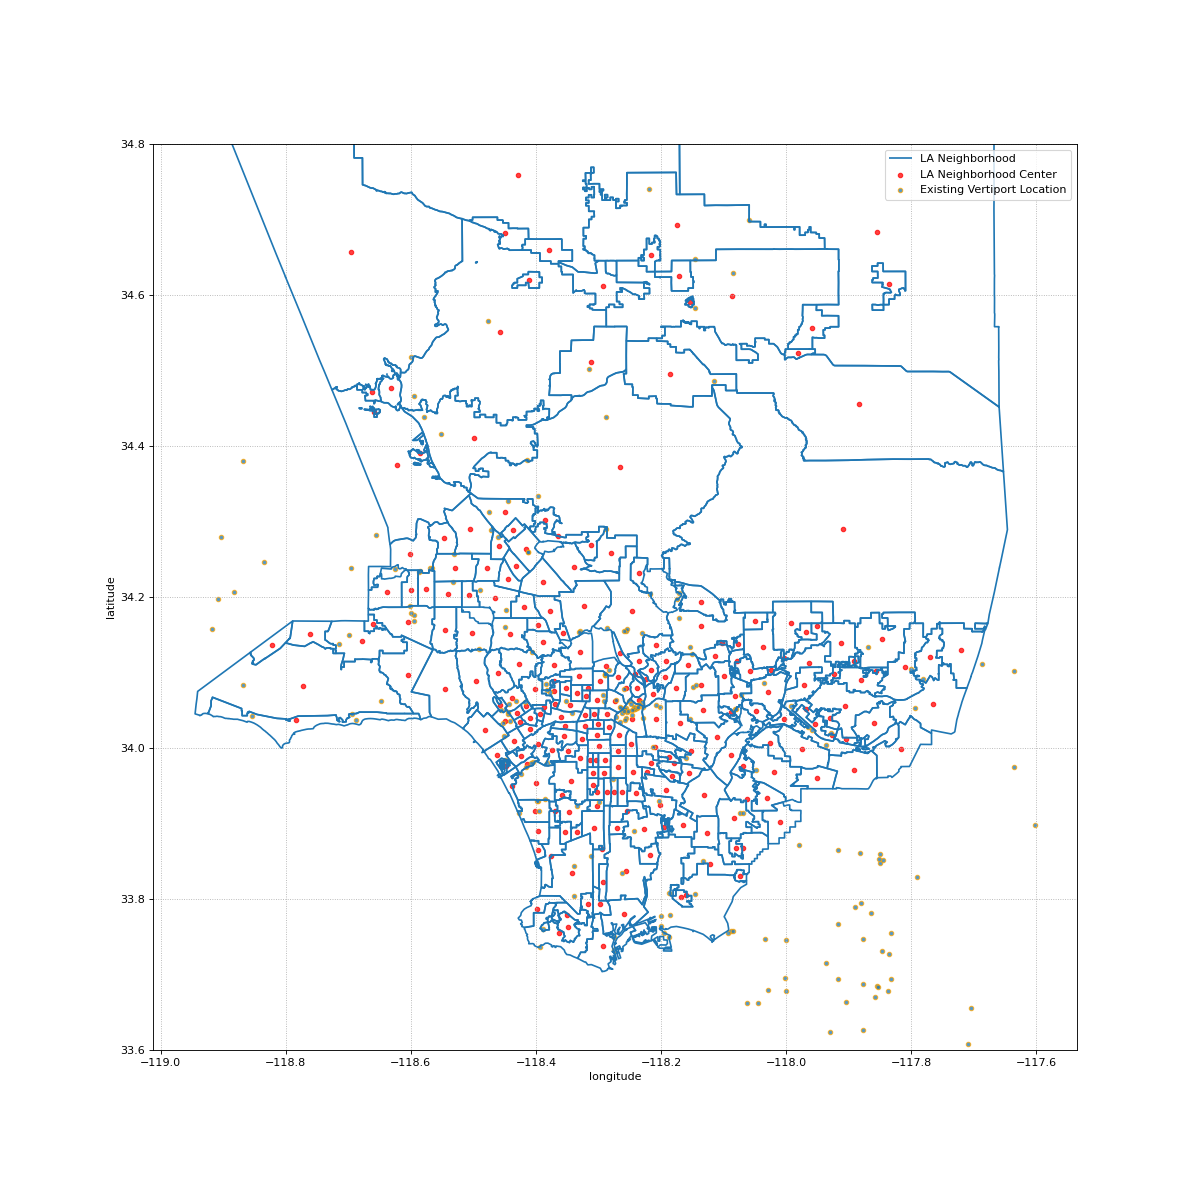
\includegraphics[width=0.8\textwidth]{proj01.png}
\vspace*{-10mm}
\caption{Los Angeles Neighborhood Centroids and Boundaries, Overlay with Available Vertiports }
\label{fig:proj01}
\end{figure}

As previously mentioned, these yellow dots correspond to the initialization locations of our cluster centers, and our goal for the clustering analysis is to cluster the red-dots by roughly equivalent population regions.

\subsubsection{Incorporating Commute Data: Exponential Smoothing}

Now, before we began our clustering analysis, we asked if we should weigh our graph by incorporating average commute times of our different neighborhoods, under the assumption that an individual forced to travel heavily-trafficked roadways would be more inclined to utilize alternative transportation.

To meet this goal, we used the U.S. Census Bureau's PUMA data from 2019 to identify commuting patterns for the LA-area in 2019. The data was reported without even partitions, so the first step was to re-sample the data set on a 10 minute interval. This resulted in many missing data points, so we decided to implement an exponential smoothing algorithm looking specifically at the morning commute hours (2 A.M. to 12 P.M.) to approximate the missing data points.

An exponential smoothing algorithm was chosen for this analysis it was a time series data set without a seasonal or trend component, since it asked only for respondents to report their average commute length at the average time they left home every morning. This analysis allowed us to utilize the existing data to approximate a smoothed model for commute lengths in each neighborhood. The smoothing parameter was varied (from 0.1 to 1) to determine the optimal level of smoothing to minimize the Sum of Squared Errors between the reported data and the fitted data.

\begin{figure}[ht]
\centering
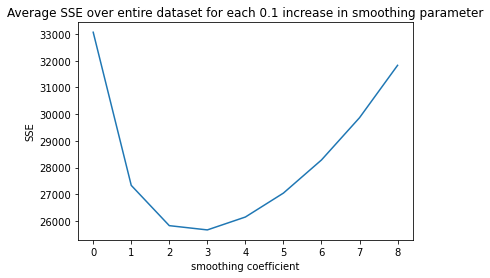
\includegraphics[width=0.8\textwidth]{proj05.png}
\vspace*{-10mm}
\caption{Average SSE for commute data }
\label{fig:proj01}
\end{figure}

Unfortunately, the data set was not dense enough to yield results that could impact this analysis. This is likely due to a few factors. First, the time series analysis required data imputation to fill out the missing values in the data set. 10 minute intervals were chosen because that level of specificity was utilized during peak commute hours, where commutes varied the greatest. However, this was a small portion of the overall data set, so the model relied on a large percentage of imputed values, sometimes upwards of 40\% of the data.

Realizing that this created an inaccurate data set, the model was also run using 0 values for missing data, and while this created more realistic approximation, it artificially lowered commute times. While this information have been scaled based on the percentage of 0 data imputed into the calculation, the sparsity of the data set lead to real difficulties in approximating the actual commutes the people of LA experience.

Ultimately, it was shown to have little effect on the analysis. The error associated with attempting to incorporate commute data into the analysis was not worth attempting to weigh each data point with the average length of the commute. Additionally, only a small subset of the roughly 270 neighborhoods in LA correlated to the PUMA data set. A regression analysis was considered to impute average length of commute for the remaining data types, however given the size of the prediction set, the inaccuracies in the underlying training data, and the lack of relevant features to use for prediction, this approach was scrapped from the project. However, the analysis did provide a distribution of approximate travel times that were sampled during the optimization routine.

As a result of this analysis, we included a term in the optimization algorithm that would favor longer routes due to the increase in revenue per passenger-mile and as a proxy for commute times, since larger distances would generally correlate to longer drive times, even though that analysis ignores .

\subsubsection{ISOMAP and Kmeans}
In order to optimize the selected vertiport locations, we chose to utilize an ISOMAP algorithm to connect discrete nodes within the graph based on the range capabilities of the aircraft. 

We began by constructing a weighted nearest neighbor graph, given by matrix $D\in R^{m\times m}$, and
\[
D_{ij} = ||x_i - x_j||_d \qquad d \text{ is geographical distance between pair of centroids}
\]

Once the graph was built, we applied the ISOMAP transformation on neighborhood centroids to take account for the geographical distance between nodes. In order to determine optimal number of clusters for great Los Angeles area, we used K-Means algorithm, and plot sum of squared distance vs. number of clusters, K, for a range of K's from 1 to 20. From Figure \ref{fig:proj02}, elbow point seems to happen between $K=5$ and $K=10$.

\begin{figure}[ht]
\centering
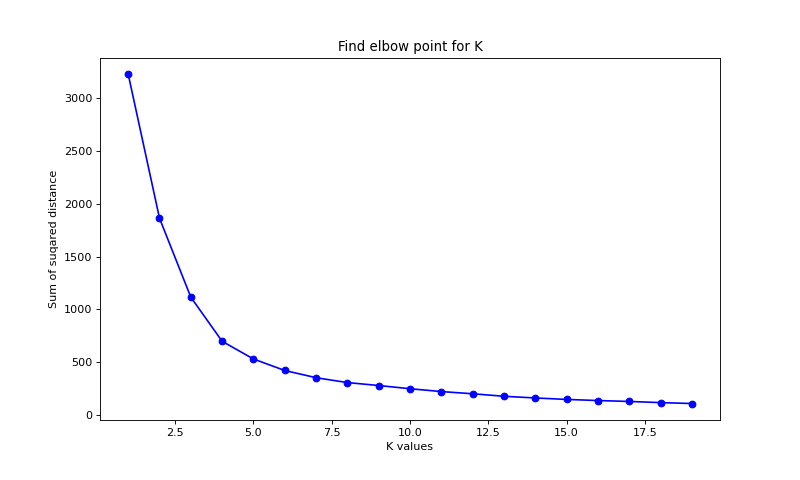
\includegraphics[width=0.8\textwidth]{proj02.png}
\vspace*{-10mm}
\caption{Find Optimal Number of Clusters}
\label{fig:proj02}
\end{figure}

Once we narrowed in on a range with an acceptable sum of squared distance, we examined a few clustering configurations for $K=5$, $K=7$ and $K=10$, as shown in Figure \ref{fig:proj03}. 

In the end, we chose to proceed with 10 cluster locations. Although the sum of squared distances decreases with more vertiports, we also need to consider the business constraints. Establishing vertiport operations is money and time intensive, so for an initial operational model, 10 locations balances cost with access to population centers in a way that encourages the use of the platforms. Additionally, we found that the optimal clustering configuration represented both urban and suburban areas, meaning that we were effective in capturing regular commute patterns and enabled a market where individuals from suburban "bedding" communities into urban centers where they otherwise would have had to drive. 

\begin{figure}[ht]
\centering
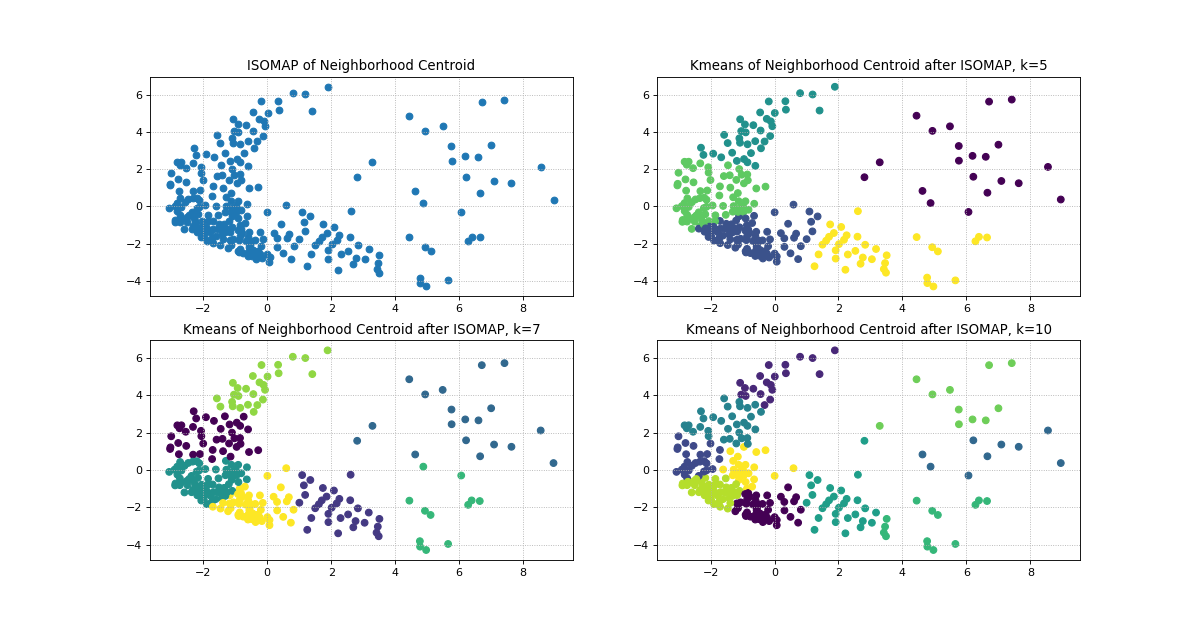
\includegraphics[width=0.9\textwidth]{proj03.png}
\vspace*{-10mm}
\caption{Different clustering results on ISOMAP of Centroids }
\label{fig:proj03}
\end{figure}

Once we established $K=10$ clusters, assign each neighborhood with its cluster label, and computed geographical cluster centers as shown in Figure \ref{fig:proj04}. Note that the mapping is color coded by population percentile, which shows that there is a higher density of cluster centers in higher populated areas, which makes sense for commuting needs.

\begin{figure}[ht]
\centering
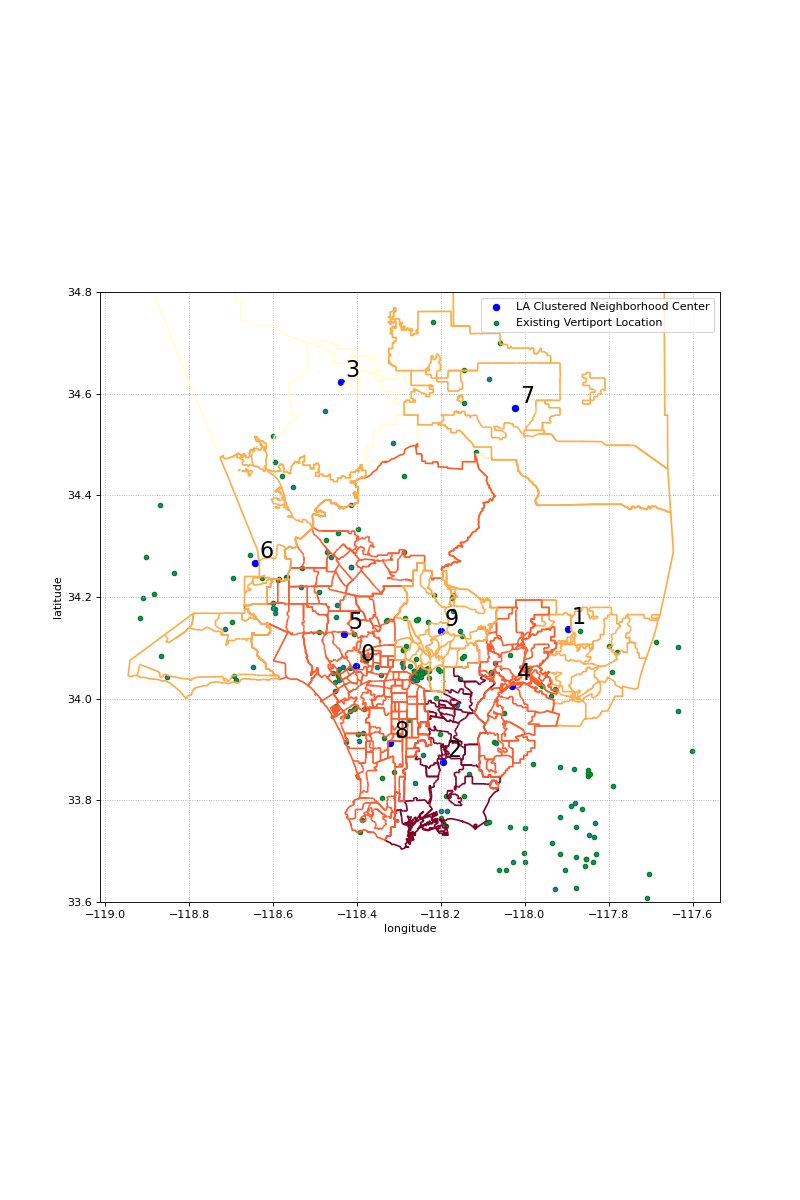
\includegraphics[width=0.8\textwidth]{proj04.png}
\vspace*{-45mm}
\caption{10 Cluster Centroids on LA Area, with Population Percentile Overlay }
\label{fig:proj04}
\end{figure}

\subsection{Optimization}

Once the ISOMAP and K-Means algorithms helped us to establish our vertiport locations, we needed to understand what the expected profitability of the operation would be. To do so, we utilized our optimized cluster centers and built a routine that would determine the optimal volume of operations, given expected capital expenditure constraints and expected design choices. 

Although we determined that K=10 is the optimal number of clusters, the graph showed that K=5-10 were all viable. Because of that, the optimization routine was run for K=5 though K=10 to determine how cluster size impacted profitability.

Industry surveys have shown typical configurations and expense models which can be viewed in Table 1 below. Additional assumptions in building the optimization problem are detailed below. Python package PuLP was utilized to develop the optimization routine.

Assumptions
\begin{enumerate}
  \item Commuters in each clusters have equal probability travel to other clusters
  \item Operation profit per passenger per mile is roughly estimated without large scale data
  \item All existing vertiports are available to use or rent
  \item Both existing and new vertiports have same eVTOL capacity
  \item eVTOL's can make a total of 15 flights per day
  \item Initial operations will have an initial capital investment of \$1 Billion
\end{enumerate}

Data
\[
\begin{split}
K& \qquad \text{Number of clusters we choose}\\
c_{ij}&  \qquad \text{Number of daily commuters between cluster $i$ and cluster $j$} \\
p_{ij}& \qquad \text{Percentage of commuter in cluster $i$ would choose eVTOL}\\
d_{ij}&  \qquad \text{geographical distance between cluster $i$ and cluster $j$} \\
P & \qquad \text{Net profit per passenger per mile} \\
V^{exist}_i & \qquad \text{Number of existing vertiport that cluster $i$ have} \\
V^{new}_i & \qquad \text{Number of new vertiport that cluster $i$ should have} \\
Cap^{eVTOL} & \qquad \text{Capacity of one eVTOL, how many commuters can one eVTOL hold} \\
Cap^{port} & \qquad \text{Capacity of one vertiport, how many eVTOL can one vertiport hold} \\
Cost^{eVTOL} & \qquad \text{how much does one eVTOL cost, depreciation life 10 years} \\
Cost^{Ve} & \qquad \text{how much does using/renting one existing vertiport cost, annually} \\
Cost^{Vn} & \qquad \text{how much does building one new vertiport cost, depreciation life 20 years} \\
N^{Ve}_i & \qquad \text{number of existing vertiport in cluster $i$} \\
N^{Vn}_i & \qquad \text{number of new vertiport in cluster $i$} \\
N^{r} & \qquad \text{number of round trips one eVTOL can make during commute hours} \\
B_{cap} & \qquad \text{Total Capital investment budget}
\end{split}
\]

Variable
\[
\begin{split}
x_{i}  & \qquad \text{Number of eVTOL that cluster $i$ should maintain}\\
\%_{util,i} & \qquad \text{Percent of population utilizing vertiport}\\
\end{split}
\]


Objective function is 
\[
\textbf{max} \biggl( \sum_{i=1}^K \sum_{j=1}^K c_{ij}p_{ij} d_{ij}P*\%_{util,i}- \sum_{i=1}^K\Bigl( \frac{1}{10\times365}Cost^{eVTOL}x_i + \frac{1}{365}Cost^{Ve}N^{Ve}_i + \frac{1}{20\times365}Cost^{Vn}N^{Vn}_i  \Bigl)\biggl)
\]

Subject to
\[
\begin{split}
x_i  \geq 0 &\qquad \text{number of eVTOL that each vertiport have cannot be zero}\\
Cap^{eVTOL}N^{r}x_i \geq \sum_{j=1}^K c_{ij}p_{ij}*\%_{util,i} &\qquad \text{total eVTOL capacity of cluster $i$ can satisfy eVTOL commute} \\
Cap^{port}(N^{Ve}_i+N^{Vn}_i) \geq x_i &\qquad  \text{total vertiport capacity of cluster $i$ can hold all eVTOL in cluster $i$} \\
Cost^{Ve}N^{Ve}_i + Cost^{eVTOL}x_i + Cost^{Vn}N^{Vn}_i \leq B_{cap} &\qquad  \text{Cost of vertiports and aircraft cannot exceed capital budget}\\
\end{split}
\]

\begin{table}[h!]
\centering
\caption{Table for constant parameters}
\begin{tabular}{|c c l|} 
 \hline
 Constant & Value & Description \\ [0.5ex] 
 \hline\hline
 $K$ & 10 & Number of clusters we choose \\
 $N^r$ & 15 & Number of round trips one eVTOL can make per day\\
 $P$ & \$0.5 & Net profit per passenger per mile \\ 
 $Cap^{eVTOL}$ & 4 & Capacity of one eVTOL\\
 $Cap^{port}$ & 8 & Capacity of one vertiport\\
 $Cost^{eVTOL}$ & \$1,000,000 & One eVTOL cost, depreciation life is 10 years\\
 $Cost^{Ve}$ & \$200,000 & Annual renting cost of one existing vertiport (Cap 8 eVTOL) \\
 $Cost^{Vn}$ & \$500,000 & Cost of converting airport to vertiport (Cap 8 eVTOL), depreciation life is 20 years \\ 
 $B_{cap}$ & \$1,000,000,000 & Total capital investment available\\[1ex] 
 \hline
\end{tabular}
\label{table:proj01}
\end{table}

\section{Final Results}

\begin{table}[h!]
\centering
\caption{Optimization Results by cluster size}
\begin{tabular}{|c c c c c c|} 
 \hline
Cluster Label& Percent Utilization & Total Profit & Number of Daily Flights & Number of eVTOLS \\ [0.5ex] 
 \hline\hline
	5	& 0.0 & \$0	&  0 & 0 \\
	6&	0.0328&	\$59,620&		14295 & 953\\
	7&	0.0365&	\$49,505&		14295 & 953\\
	8&	0.0943&	\$114,905&		31111, 2074\\
	9&	0.1371&	\$198,766&		42917 & 2861\\
	10&	0.1550&	\$390,096&		42932 & 2862\\ [1ex] 
 \hline
\end{tabular}
\label{table:proj02}
\end{table}


As you can see from the results above, developing a robust, profitable model for the eVTOL industry is not a trivial problem. The total daily profit for one company operating within the parameters outlined above equates to \$390,096, while only factoring in capital expenses, not wages or other costs. 

This model also ignores the very real constraint of physical land access. The model does not control for the physical positioning of the additional vertiports in the region.

The most shocking result from this analysis is the asymmetric utilization of the vertiports. Given that the clustering analysis optimizes to balance the total population equally between the clusters, the utilization is not evenly distributed.

However, this result is not all that shocking. The algoirthm tended to favor increasing operational volume between the furthest cluster pairs in the network. Without an accurate way to account for demand, this is the natural result of the algorithm.

\begin{table}[h!]
\centering
\caption{Demand for k=10}
\begin{tabular}{|c c c c|} 
 \hline
Cluster Label& New Vertiport Capacity& Number of eVTOL's Needed& Percent Utilization  \\ [0.5ex] 
 \hline\hline
0&0 & 0 & 0\\ 
1&0 & 0 & 0\\
2&0 & 0 & 0\\
3&93 & 952 & 0.0590\\
4&0 & 0 & 0\\
5&0 & 0 & 0\\
6&77 & 957 & 0.0473\\
7&91 & 953 & 0.0486\\
8&0 & 0 & 0\\
9&0 & 0 & 0\\[1ex] 
 \hline
\end{tabular}
\label{table:proj02}
\end{table}

\section{Evaluation}

Determining the utilization and profitability of an eVTOL market is extremely complex and relies on a number of competing priorities for utilization of capital investments. Our analysis utilized optimal operations locations based on a combination of ISOMAP and KMeans algorithms to develop a network to model typical operations. Then, an optimization routine took known capital expenditures, design limitations, cost models, and more to determine the expected profitability of the operations.

This model took a few liberties in the analysis that reduced the accuracy to real-world dynamics a company might expect, but does show a potential business model and builds a baseline for future operators to understand their business needs and metrics targets to achieve profitability. For example, this model assumed that consumer utilization was an independent factor, which is not truly representative of consumer sentiment and access to the technology. Initially, some small percentage of the population will be willing to utilize the platform for their commuting needs. As consumers gain acceptance of the technology, and as the cost per passenger-mile decreases, new markets open and and demand changes. Assuming that high net-worth individuals and those willing to utilize the technology were independently and identically distributed around LA is not entirely accurate. Those individuals would tend to be clustered in certain regions, and thus a more accurate model would weigh the population clusters by the wealth of the region to determine an initial model that would have better projected usage, especially during initial operations.

Additionally, as previously mentioned, average commute times were not factored into the model. One might expect that there is a direct relation between commute time and willingness to utilize eVTOL aircraft, as consumers would have to rationalize paying for the service by the expected benefit of the reduced travel time. This factor could be leveraged, along with demographic data such as wealth, in determining more accurate vertiport locations and utilization metrics.

However, the model does paint a promising picture: the LA market could support a mature eVTOL operation, based on assumed industry cost parameters and design decisions. It is not an easy endeavor, and is extremely costly, but with all new technologies, choosing a market that can sustain operations is critical to success.

This model acts as a first-glance for business leaders to determine target values for engineering leaders to target, such as expected vehicle cost and expected utilization, as well as marketing goals for consumer acceptance and demand. Optimizing between all of these parameters paint a dynamic picture that allow business leaders to choose targets that work best for their operation. 

\subsection{Future refinement}
For future considerations, there are a number of improvements that could be incorporated. For one, we have to model more realistic mobility patterns. There is likely to be asymmetric demand in the network, meaning that there will be more demand for flights into LA in the morning and out of LA in the evening. Additionally, demand between all nodes in the vertiport will not be symmetric either. There will be greater demand for suburban nodes to go to urban ones rather than other suburban nodes. This fact will have to be incorporated into future iterations to better understand how demand profiles propagate.

Additionally, other demographic factors, such as wealth, age, race, etc. should be incorporated to better model utilization of the service. Certain demographics will be more likely to utilize eVTOL aircraft, and that demand should be captured to better understand where to place vertiport locations.

Lastly, future work should incorporate second-order effects, i.e. how increased demand for eVTOL changes traffic patterns and affects the cost-benefit equation for the individual consumer. Reduced congestion leads to shorter commutes, which might drive other customers back onto the roads into an equilibrium. This effect will have to be captured to accurately determine the total addressable market. 

\pagebreak

\begin{appendix}
  \listoffigures
  \listoftables
\end{appendix}

\end{document}